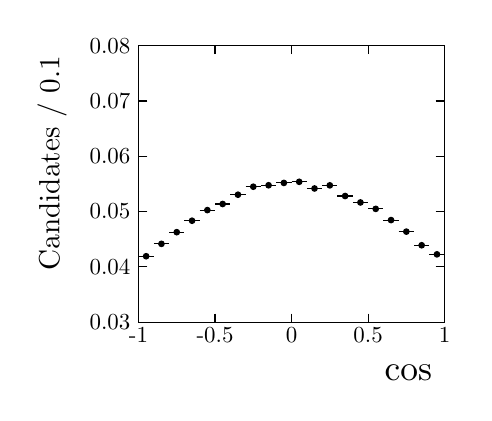
\begin{tikzpicture}
\pgfdeclareplotmark{cross} {
\pgfpathmoveto{\pgfpoint{-0.3\pgfplotmarksize}{\pgfplotmarksize}}
\pgfpathlineto{\pgfpoint{+0.3\pgfplotmarksize}{\pgfplotmarksize}}
\pgfpathlineto{\pgfpoint{+0.3\pgfplotmarksize}{0.3\pgfplotmarksize}}
\pgfpathlineto{\pgfpoint{+1\pgfplotmarksize}{0.3\pgfplotmarksize}}
\pgfpathlineto{\pgfpoint{+1\pgfplotmarksize}{-0.3\pgfplotmarksize}}
\pgfpathlineto{\pgfpoint{+0.3\pgfplotmarksize}{-0.3\pgfplotmarksize}}
\pgfpathlineto{\pgfpoint{+0.3\pgfplotmarksize}{-1.\pgfplotmarksize}}
\pgfpathlineto{\pgfpoint{-0.3\pgfplotmarksize}{-1.\pgfplotmarksize}}
\pgfpathlineto{\pgfpoint{-0.3\pgfplotmarksize}{-0.3\pgfplotmarksize}}
\pgfpathlineto{\pgfpoint{-1.\pgfplotmarksize}{-0.3\pgfplotmarksize}}
\pgfpathlineto{\pgfpoint{-1.\pgfplotmarksize}{0.3\pgfplotmarksize}}
\pgfpathlineto{\pgfpoint{-0.3\pgfplotmarksize}{0.3\pgfplotmarksize}}
\pgfpathclose
\pgfusepathqstroke
}
\pgfdeclareplotmark{cross*} {
\pgfpathmoveto{\pgfpoint{-0.3\pgfplotmarksize}{\pgfplotmarksize}}
\pgfpathlineto{\pgfpoint{+0.3\pgfplotmarksize}{\pgfplotmarksize}}
\pgfpathlineto{\pgfpoint{+0.3\pgfplotmarksize}{0.3\pgfplotmarksize}}
\pgfpathlineto{\pgfpoint{+1\pgfplotmarksize}{0.3\pgfplotmarksize}}
\pgfpathlineto{\pgfpoint{+1\pgfplotmarksize}{-0.3\pgfplotmarksize}}
\pgfpathlineto{\pgfpoint{+0.3\pgfplotmarksize}{-0.3\pgfplotmarksize}}
\pgfpathlineto{\pgfpoint{+0.3\pgfplotmarksize}{-1.\pgfplotmarksize}}
\pgfpathlineto{\pgfpoint{-0.3\pgfplotmarksize}{-1.\pgfplotmarksize}}
\pgfpathlineto{\pgfpoint{-0.3\pgfplotmarksize}{-0.3\pgfplotmarksize}}
\pgfpathlineto{\pgfpoint{-1.\pgfplotmarksize}{-0.3\pgfplotmarksize}}
\pgfpathlineto{\pgfpoint{-1.\pgfplotmarksize}{0.3\pgfplotmarksize}}
\pgfpathlineto{\pgfpoint{-0.3\pgfplotmarksize}{0.3\pgfplotmarksize}}
\pgfpathclose
\pgfusepathqfillstroke
}
\pgfdeclareplotmark{newstar} {
\pgfpathmoveto{\pgfqpoint{0pt}{\pgfplotmarksize}}
\pgfpathlineto{\pgfqpointpolar{44}{0.5\pgfplotmarksize}}
\pgfpathlineto{\pgfqpointpolar{18}{\pgfplotmarksize}}
\pgfpathlineto{\pgfqpointpolar{-20}{0.5\pgfplotmarksize}}
\pgfpathlineto{\pgfqpointpolar{-54}{\pgfplotmarksize}}
\pgfpathlineto{\pgfqpointpolar{-90}{0.5\pgfplotmarksize}}
\pgfpathlineto{\pgfqpointpolar{234}{\pgfplotmarksize}}
\pgfpathlineto{\pgfqpointpolar{198}{0.5\pgfplotmarksize}}
\pgfpathlineto{\pgfqpointpolar{162}{\pgfplotmarksize}}
\pgfpathlineto{\pgfqpointpolar{134}{0.5\pgfplotmarksize}}
\pgfpathclose
\pgfusepathqstroke
}
\pgfdeclareplotmark{newstar*} {
\pgfpathmoveto{\pgfqpoint{0pt}{\pgfplotmarksize}}
\pgfpathlineto{\pgfqpointpolar{44}{0.5\pgfplotmarksize}}
\pgfpathlineto{\pgfqpointpolar{18}{\pgfplotmarksize}}
\pgfpathlineto{\pgfqpointpolar{-20}{0.5\pgfplotmarksize}}
\pgfpathlineto{\pgfqpointpolar{-54}{\pgfplotmarksize}}
\pgfpathlineto{\pgfqpointpolar{-90}{0.5\pgfplotmarksize}}
\pgfpathlineto{\pgfqpointpolar{234}{\pgfplotmarksize}}
\pgfpathlineto{\pgfqpointpolar{198}{0.5\pgfplotmarksize}}
\pgfpathlineto{\pgfqpointpolar{162}{\pgfplotmarksize}}
\pgfpathlineto{\pgfqpointpolar{134}{0.5\pgfplotmarksize}}
\pgfpathclose
\pgfusepathqfillstroke
}
\definecolor{c}{rgb}{1,1,1};
\draw [color=c, fill=c] (0.1,4.72095) rectangle (4.9,9.16419);
\draw [color=c, fill=c] (0.772,5.43186) rectangle (4.66,8.94203);
\definecolor{c}{rgb}{0,0,0};
\draw [c] (0.772,5.43186) -- (0.772,8.94203) -- (4.66,8.94203) -- (4.66,5.43186) -- (0.772,5.43186);
\draw [c,line width=0.4] (0.8692,6.25424) -- (0.8692,6.26862);
\draw [c,line width=0.4] (0.8692,6.26862) -- (0.8692,6.28299);
\draw [c,line width=0.4] (0.772,6.26862) -- (0.8692,6.26862);
\draw [c,line width=0.4] (0.8692,6.26862) -- (0.9664,6.26862);
\foreach \P in {(0.8692,6.26862)}{\draw[mark options={color=c,fill=c},mark size=1.201201pt,mark=*,mark size=1pt] plot coordinates {\P};}
\draw [c,line width=0.4] (1.0636,6.41098) -- (1.0636,6.42573);
\draw [c,line width=0.4] (1.0636,6.42573) -- (1.0636,6.44048);
\draw [c,line width=0.4] (0.9664,6.42573) -- (1.0636,6.42573);
\draw [c,line width=0.4] (1.0636,6.42573) -- (1.1608,6.42573);
\foreach \P in {(1.0636,6.42573)}{\draw[mark options={color=c,fill=c},mark size=1.201201pt,mark=*,mark size=1pt] plot coordinates {\P};}
\draw [c,line width=0.4] (1.258,6.55876) -- (1.258,6.57386);
\draw [c,line width=0.4] (1.258,6.57386) -- (1.258,6.58896);
\draw [c,line width=0.4] (1.1608,6.57386) -- (1.258,6.57386);
\draw [c,line width=0.4] (1.258,6.57386) -- (1.3552,6.57386);
\foreach \P in {(1.258,6.57386)}{\draw[mark options={color=c,fill=c},mark size=1.201201pt,mark=*,mark size=1pt] plot coordinates {\P};}
\draw [c,line width=0.4] (1.4524,6.70396) -- (1.4524,6.71939);
\draw [c,line width=0.4] (1.4524,6.71939) -- (1.4524,6.73483);
\draw [c,line width=0.4] (1.3552,6.71939) -- (1.4524,6.71939);
\draw [c,line width=0.4] (1.4524,6.71939) -- (1.5496,6.71939);
\foreach \P in {(1.4524,6.71939)}{\draw[mark options={color=c,fill=c},mark size=1.201201pt,mark=*,mark size=1pt] plot coordinates {\P};}
\draw [c,line width=0.4] (1.6468,6.83858) -- (1.6468,6.85432);
\draw [c,line width=0.4] (1.6468,6.85432) -- (1.6468,6.87006);
\draw [c,line width=0.4] (1.5496,6.85432) -- (1.6468,6.85432);
\draw [c,line width=0.4] (1.6468,6.85432) -- (1.744,6.85432);
\foreach \P in {(1.6468,6.85432)}{\draw[mark options={color=c,fill=c},mark size=1.201201pt,mark=*,mark size=1pt] plot coordinates {\P};}
\draw [c,line width=0.4] (1.8412,6.91599) -- (1.8412,6.9319);
\draw [c,line width=0.4] (1.8412,6.9319) -- (1.8412,6.94781);
\draw [c,line width=0.4] (1.744,6.9319) -- (1.8412,6.9319);
\draw [c,line width=0.4] (1.8412,6.9319) -- (1.9384,6.9319);
\foreach \P in {(1.8412,6.9319)}{\draw[mark options={color=c,fill=c},mark size=1.201201pt,mark=*,mark size=1pt] plot coordinates {\P};}
\draw [c,line width=0.4] (2.0356,7.03346) -- (2.0356,7.04963);
\draw [c,line width=0.4] (2.0356,7.04963) -- (2.0356,7.0658);
\draw [c,line width=0.4] (1.9384,7.04963) -- (2.0356,7.04963);
\draw [c,line width=0.4] (2.0356,7.04963) -- (2.1328,7.04963);
\foreach \P in {(2.0356,7.04963)}{\draw[mark options={color=c,fill=c},mark size=1.201201pt,mark=*,mark size=1pt] plot coordinates {\P};}
\draw [c,line width=0.4] (2.23,7.13489) -- (2.23,7.15128);
\draw [c,line width=0.4] (2.23,7.15128) -- (2.23,7.16767);
\draw [c,line width=0.4] (2.1328,7.15128) -- (2.23,7.15128);
\draw [c,line width=0.4] (2.23,7.15128) -- (2.3272,7.15128);
\foreach \P in {(2.23,7.15128)}{\draw[mark options={color=c,fill=c},mark size=1.201201pt,mark=*,mark size=1pt] plot coordinates {\P};}
\draw [c,line width=0.4] (2.4244,7.15325) -- (2.4244,7.16968);
\draw [c,line width=0.4] (2.4244,7.16968) -- (2.4244,7.1861);
\draw [c,line width=0.4] (2.3272,7.16968) -- (2.4244,7.16968);
\draw [c,line width=0.4] (2.4244,7.16968) -- (2.5216,7.16968);
\foreach \P in {(2.4244,7.16968)}{\draw[mark options={color=c,fill=c},mark size=1.201201pt,mark=*,mark size=1pt] plot coordinates {\P};}
\draw [c,line width=0.4] (2.6188,7.18316) -- (2.6188,7.19965);
\draw [c,line width=0.4] (2.6188,7.19965) -- (2.6188,7.21614);
\draw [c,line width=0.4] (2.5216,7.19965) -- (2.6188,7.19965);
\draw [c,line width=0.4] (2.6188,7.19965) -- (2.716,7.19965);
\foreach \P in {(2.6188,7.19965)}{\draw[mark options={color=c,fill=c},mark size=1.201201pt,mark=*,mark size=1pt] plot coordinates {\P};}
\draw [c,line width=0.4] (2.8132,7.19717) -- (2.8132,7.21369);
\draw [c,line width=0.4] (2.8132,7.21369) -- (2.8132,7.23021);
\draw [c,line width=0.4] (2.716,7.21369) -- (2.8132,7.21369);
\draw [c,line width=0.4] (2.8132,7.21369) -- (2.9104,7.21369);
\foreach \P in {(2.8132,7.21369)}{\draw[mark options={color=c,fill=c},mark size=1.201201pt,mark=*,mark size=1pt] plot coordinates {\P};}
\draw [c,line width=0.4] (3.0076,7.11255) -- (3.0076,7.12889);
\draw [c,line width=0.4] (3.0076,7.12889) -- (3.0076,7.14523);
\draw [c,line width=0.4] (2.9104,7.12889) -- (3.0076,7.12889);
\draw [c,line width=0.4] (3.0076,7.12889) -- (3.1048,7.12889);
\foreach \P in {(3.0076,7.12889)}{\draw[mark options={color=c,fill=c},mark size=1.201201pt,mark=*,mark size=1pt] plot coordinates {\P};}
\draw [c,line width=0.4] (3.202,7.15241) -- (3.202,7.16883);
\draw [c,line width=0.4] (3.202,7.16883) -- (3.202,7.18526);
\draw [c,line width=0.4] (3.1048,7.16883) -- (3.202,7.16883);
\draw [c,line width=0.4] (3.202,7.16883) -- (3.2992,7.16883);
\foreach \P in {(3.202,7.16883)}{\draw[mark options={color=c,fill=c},mark size=1.201201pt,mark=*,mark size=1pt] plot coordinates {\P};}
\draw [c,line width=0.4] (3.3964,7.01693) -- (3.3964,7.03306);
\draw [c,line width=0.4] (3.3964,7.03306) -- (3.3964,7.04919);
\draw [c,line width=0.4] (3.2992,7.03306) -- (3.3964,7.03306);
\draw [c,line width=0.4] (3.3964,7.03306) -- (3.4936,7.03306);
\foreach \P in {(3.3964,7.03306)}{\draw[mark options={color=c,fill=c},mark size=1.201201pt,mark=*,mark size=1pt] plot coordinates {\P};}
\draw [c,line width=0.4] (3.5908,6.93553) -- (3.5908,6.95148);
\draw [c,line width=0.4] (3.5908,6.95148) -- (3.5908,6.96744);
\draw [c,line width=0.4] (3.4936,6.95148) -- (3.5908,6.95148);
\draw [c,line width=0.4] (3.5908,6.95148) -- (3.688,6.95148);
\foreach \P in {(3.5908,6.95148)}{\draw[mark options={color=c,fill=c},mark size=1.201201pt,mark=*,mark size=1pt] plot coordinates {\P};}
\draw [c,line width=0.4] (3.7852,6.85406) -- (3.7852,6.86984);
\draw [c,line width=0.4] (3.7852,6.86984) -- (3.7852,6.88561);
\draw [c,line width=0.4] (3.688,6.86984) -- (3.7852,6.86984);
\draw [c,line width=0.4] (3.7852,6.86984) -- (3.8824,6.86984);
\foreach \P in {(3.7852,6.86984)}{\draw[mark options={color=c,fill=c},mark size=1.201201pt,mark=*,mark size=1pt] plot coordinates {\P};}
\draw [c,line width=0.4] (3.9796,6.71208) -- (3.9796,6.72754);
\draw [c,line width=0.4] (3.9796,6.72754) -- (3.9796,6.74299);
\draw [c,line width=0.4] (3.8824,6.72754) -- (3.9796,6.72754);
\draw [c,line width=0.4] (3.9796,6.72754) -- (4.0768,6.72754);
\foreach \P in {(3.9796,6.72754)}{\draw[mark options={color=c,fill=c},mark size=1.201201pt,mark=*,mark size=1pt] plot coordinates {\P};}
\draw [c,line width=0.4] (4.174,6.5659) -- (4.174,6.58102);
\draw [c,line width=0.4] (4.174,6.58102) -- (4.174,6.59614);
\draw [c,line width=0.4] (4.0768,6.58102) -- (4.174,6.58102);
\draw [c,line width=0.4] (4.174,6.58102) -- (4.2712,6.58102);
\foreach \P in {(4.174,6.58102)}{\draw[mark options={color=c,fill=c},mark size=1.201201pt,mark=*,mark size=1pt] plot coordinates {\P};}
\draw [c,line width=0.4] (4.3684,6.39312) -- (4.3684,6.40783);
\draw [c,line width=0.4] (4.3684,6.40783) -- (4.3684,6.42254);
\draw [c,line width=0.4] (4.2712,6.40783) -- (4.3684,6.40783);
\draw [c,line width=0.4] (4.3684,6.40783) -- (4.4656,6.40783);
\foreach \P in {(4.3684,6.40783)}{\draw[mark options={color=c,fill=c},mark size=1.201201pt,mark=*,mark size=1pt] plot coordinates {\P};}
\draw [c,line width=0.4] (4.5628,6.27791) -- (4.5628,6.29235);
\draw [c,line width=0.4] (4.5628,6.29235) -- (4.5628,6.30678);
\draw [c,line width=0.4] (4.4656,6.29235) -- (4.5628,6.29235);
\draw [c,line width=0.4] (4.5628,6.29235) -- (4.66,6.29235);
\foreach \P in {(4.5628,6.29235)}{\draw[mark options={color=c,fill=c},mark size=1.201201pt,mark=*,mark size=1pt] plot coordinates {\P};}
\draw [c,line width=0.4] (0.772,5.43186) -- (4.66,5.43186);
\draw [anchor= east] (4.66,4.78493) node[scale=1.28062, rotate=0]{$\cos\thetamu$};
\draw [c,line width=0.4] (0.772,5.53984) -- (0.772,5.43186);
\draw [c,line width=0.4] (1.744,5.53984) -- (1.744,5.43186);
\draw [c,line width=0.4] (2.716,5.53984) -- (2.716,5.43186);
\draw [c,line width=0.4] (3.688,5.53984) -- (3.688,5.43186);
\draw [c,line width=0.4] (4.66,5.53984) -- (4.66,5.43186);
\draw [anchor=base] (0.772,5.17416) node[scale=0.828637, rotate=0]{-1};
\draw [anchor=base] (1.744,5.17416) node[scale=0.828637, rotate=0]{-0.5};
\draw [anchor=base] (2.716,5.17416) node[scale=0.828637, rotate=0]{0};
\draw [anchor=base] (3.688,5.17416) node[scale=0.828637, rotate=0]{0.5};
\draw [anchor=base] (4.66,5.17416) node[scale=0.828637, rotate=0]{1};
\draw [c,line width=0.4] (0.772,8.94203) -- (4.66,8.94203);
\draw [c,line width=0.4] (0.772,8.83406) -- (0.772,8.94203);
\draw [c,line width=0.4] (1.744,8.83406) -- (1.744,8.94203);
\draw [c,line width=0.4] (2.716,8.83406) -- (2.716,8.94203);
\draw [c,line width=0.4] (3.688,8.83406) -- (3.688,8.94203);
\draw [c,line width=0.4] (4.66,8.83406) -- (4.66,8.94203);
\draw [c,line width=0.4] (0.772,5.43186) -- (0.772,8.94203);
\draw [anchor= east] (-0.32624,8.94203) node[scale=1.05463, rotate=90]{Candidates / 0.1};
\draw [c,line width=0.4] (0.88576,5.43186) -- (0.772,5.43186);
\draw [c,line width=0.4] (0.88576,6.1339) -- (0.772,6.1339);
\draw [c,line width=0.4] (0.88576,6.83593) -- (0.772,6.83593);
\draw [c,line width=0.4] (0.88576,7.53796) -- (0.772,7.53796);
\draw [c,line width=0.4] (0.88576,8.24) -- (0.772,8.24);
\draw [c,line width=0.4] (0.88576,8.94203) -- (0.772,8.94203);
\draw [anchor= east] (0.772,5.43186) node[scale=0.828637, rotate=0]{0.03};
\draw [anchor= east] (0.772,6.1339) node[scale=0.828637, rotate=0]{0.04};
\draw [anchor= east] (0.772,6.83593) node[scale=0.828637, rotate=0]{0.05};
\draw [anchor= east] (0.772,7.53796) node[scale=0.828637, rotate=0]{0.06};
\draw [anchor= east] (0.772,8.24) node[scale=0.828637, rotate=0]{0.07};
\draw [anchor= east] (0.772,8.94203) node[scale=0.828637, rotate=0]{0.08};
\draw [c,line width=0.4] (4.66,5.43186) -- (4.66,8.94203);
\draw [c,line width=0.4] (4.54624,5.43186) -- (4.66,5.43186);
\draw [c,line width=0.4] (4.54624,6.1339) -- (4.66,6.1339);
\draw [c,line width=0.4] (4.54624,6.83593) -- (4.66,6.83593);
\draw [c,line width=0.4] (4.54624,7.53796) -- (4.66,7.53796);
\draw [c,line width=0.4] (4.54624,8.24) -- (4.66,8.24);
\draw [c,line width=0.4] (4.54624,8.94203) -- (4.66,8.94203);
\end{tikzpicture}
